\chapter{Singly Balanced versus Single-ended FET Mixer}\label{sec:endvsbal}
	\section{Introduction}
		This topic is not easily covered and strict limitations are made to only consider the circumstances in this project. Both a single-balanced and a single-ended FET resistive mixer are implemented using ideal components to form groundwork to decide which mixer topology is the best choice. The main focus is the linearity ($IIP_3$) of the mixers. From the implementations, the single-ended mixer is eventually selected. This is due to its simplicity and sufficient performance.

	\section{Single-ended mixer}
		A single-ended cold FET mixer is the simplest version of a FET mixer possible. It is simply a FET with the LO connected to the gate and the RF and IF connected to the drain. Besides the FET, there is need for a bias network and for a diplexer to separate the two signals on the drain.

		The single-ended mixer is implemented with an ideal frequency split, acting as the diplexer separating the RF and the IF on the drain of the mixing FET. The gate of the FET is biased via an ideal RF-choke to $v_{gs}=\unit[-1]{V}$. The FET model used is the UMS PPH25 NCF (non-linear cold FET), which is the only non-ideal component in the design.

	\section{Balanced mixer}
		\subsection{Concept}
			Balanced mixers promise better linearity and suppression of spurious responses. There are different topologies but all of them require at least one balun and usually a stronger LO drive since two or more FETs are used. The performance of balanced mixers largely depends on the baluns. Thus, large effort is put into the design of these. An obvious drawback is the bulky nature of these balanced to unbalanced transition.

			The ideal implementation of a balanced mixer uses two perfect 180$^\circ$ baluns, with the ability to control the loss and phase imbalance. They are placed at the LO-port and the IF-port. The two NCF FETs required in a balanced setup are both biased with $v_{gs}=\unit[-1]{V}$, just as the unbalanced mixer. No filters are used.

		\subsection{Baluns}
			The purpose of baluns is to convert an unbalanced signal (a single signal in reference to ground) into its balanced counterparts (in which there are two signals, usually described as positive and negative) or vice versa. As such, they are usually three-ports, receiving a signal relative ground on one port and output the balanced signal on the two remaining ports.

			Baluns can be active, lumped or distributed. Because of the size of distributed baluns at these frequencies, they are not considered for this project. Active baluns use FETs and have gain.

			The layout and performance of an implemented lumped element balun is shown in \autoref{fig:balun_lumped}.\autocite{kuylenstierna04} The construction is quite simple, but the bandwidth is not large enough for the LO-signal. The amplitude difference is rather large as $f_{LO}$ increases, which impacts on the performance of a balanced mixer.

			\begin{figure}[hpt!]
				\centering
				\subfloat[][]{
					\includegraphics[width=0.5\textwidth]{fig/mixercomp/balun_lumped_layout}
					\label{fig:balun_lumped_layout}
				}
				\subfloat[][]{
					\includerect{0.5\textwidth}{fig/mixercomp/balun_lumped_performance}
					\label{fig:balun_lumped_performance}
				}
				\caption{\subref{fig:balun_lumped_layout} The layout and \subref{fig:balun_lumped_performance} the simulated performance of a simple lumped element 180$^\circ$ balun.}\label{fig:balun_lumped}
			\end{figure}
%			\begin{figure}[hbt!]
%				\centering
%				\includegraphics[width=0.8\textwidth]{fig/amplifiers/lo/balun_lumped_layout}
%				\caption{A lumped $180^\circ$ balun.}\label{fig:balun_lumped_layout}
%			\end{figure}
%
%			\begin{figure}[hbt!]
%				\centering
%				\includerect{0.7\textwidth}{fig/amplifiers/lo/balun_lumped_performance}
%				\caption{Lumped balun's performance. The amplitude bandwidth is rather narrow.}\label{fig:balun_lumped_performance}
%			\end{figure}

	\section{Results}
		A phase shift in the baluns of a singly balanced mixer does not have as big an impact on linearity as expected. $IIP_3$ is almost constant for a 10$^\circ$ phase difference in the balanced signal. The linearity is however very sensitive to the loss in the baluns, as shown in \autoref{fig:iip3balun}. No component in the single-ended mixer has been observed to affect the $IIP_3$ in a similar manner.

		\begin{figure}[hbt!]
			\centering
			\includerect{0.6\textwidth}{fig/mixercomp/iip3balvsbalun}
			\caption{$IIP_3$ of the singly balanced mixer versus the loss in one of the two baluns. The affect on $IIP_3$ is the same regardless of in which balun the losses are present. In this case the other balun is set to zero loss. The LO power is \unit[12]{dBm} and the signal is matched to \unit[50]{$\Omega$} (i.e. not matched to the mixer).}\label{fig:iip3balun}
		\end{figure}

		In \autoref{fig:iip3comparison}, the $IIP_3$ is compared between the two topologies. For the balanced mixer, there is a \unit[2]{dB} loss applied to both baluns. This is a loss that is considered reasonable in a non-ideal implementation. No comparison of conversion gain between the topologies has been performed, as the filter structures that produce most losses are ideal and different for the two mixers.

		\begin{figure}[hpt!]
			\centering
			\subfloat[][]{
				\includerect{0.5\textwidth}{fig/mixercomp/iip3singlevslo}
				\label{fig:iip3singleended}
			}
			\subfloat[][]{
				\includerect{0.5\textwidth}{fig/mixercomp/iip3balvslo}
				\label{fig:iip3balanced}
			}
			\caption{$IIP_3$ for \subref{fig:iip3singleended} the single-ended mixer and \subref{fig:iip3balanced} the singly balanced mixer. Here the balanced mixer has a realistic \unit[2]{dB} loss in each of its two baluns. The FET linearity decreases in both cases, as the LO power exceeds \unit[14]{dBm}. The LO is matched to \unit[50]{$\Omega$}, which is different from the gate impedance.}\label{fig:iip3comparison}
		\end{figure}

	\section{Conclusion}
		From the simulation results of the ideal mixers, it is evident that a balanced structure gives the highest $IIP_3$. However, for small losses in the baluns, the performance drop rapidly and becomes comparable to the single-ended mixer. As the LO-signal has \unit[500]{MHz} bandwidth, it is probable that a balun that can handle such a bandwidth becomes rather complex and thus has considerable losses. An IF-balun would also have some losses, although not as much as the LO-balun would. Another important issue to take into consideration is the large space that baluns require on an MMIC at these frequencies.

		This leads to the conclusion that the simple unbalanced single-ended design provides good enough performance, while at the same time being very space efficient and easy to implement.
